\documentclass{article}
\usepackage{fancyhdr}
\usepackage{extramarks}
\usepackage{amsmath}
\usepackage{amssymb}
\usepackage{enumerate}
\usepackage{graphicx}
\usepackage{pgfplotstable}
\usepackage{listings}
\usepackage{braket}
\usepackage{float}
\usepackage{subfig}
\lstset{framexleftmargin=5mm, frame=shadowbox, rulesepcolor=\color{blue}}


\topmargin=-0.45in
\evensidemargin=0in
\oddsidemargin=0in
\textwidth=6.5in
\textheight=9.0in
\headsep=0.25in

\linespread{1.1}

\pagestyle{fancy}
\lhead{\hmwkAuthorName}
\chead{\hmwkClass\ : \hmwkTitle}
\rhead{\firstxmark}
\lfoot{\lastxmark}
\cfoot{\thepage}

\renewcommand\headrulewidth{0.4pt}
\renewcommand\footrulewidth{0.4pt}

\setlength\parindent{24pt}

%
% Create Problem Sections
%

\newcommand{\enterProblemHeader}[1]{
    \nobreak\extramarks{}{Problem \arabic{#1} continued on next page\ldots}\nobreak{}
    \nobreak\extramarks{Problem \arabic{#1} (continued)}{Problem \arabic{#1} continued on next page\ldots}\nobreak{}
}

\newcommand{\exitProblemHeader}[1]{
    \nobreak\extramarks{Problem \arabic{#1} (continued)}{Problem \arabic{#1} continued on next page\ldots}\nobreak{}
    \stepcounter{#1}
    \nobreak\extramarks{Problem \arabic{#1}}{}\nobreak{}
}

\setcounter{secnumdepth}{0}
\newcounter{partCounter}
\newcounter{homeworkProblemCounter}
\setcounter{homeworkProblemCounter}{1}
\nobreak\extramarks{Problem \arabic{homeworkProblemCounter}}{}\nobreak{}

%
% Homework Problem Environment
%
% This environment takes an optional argument. When given, it will adjust the
% problem counter. This is useful for when the problems given for your
% assignment aren't sequential. See the last 3 problems of this template for an
% example.
%
\newenvironment{homeworkProblem}[1][-1]{
    \ifnum#1>0
        \setcounter{homeworkProblemCounter}{#1}
    \fi
    \section{Problem \arabic{homeworkProblemCounter}}
    \setcounter{partCounter}{1}
    \enterProblemHeader{homeworkProblemCounter}
}{
    \exitProblemHeader{homeworkProblemCounter}
}

%
% Homework Details
%   - Title
%   - Due date
%   - Class
%   - Section/Time
%   - Instructor
%   - Author
%

\newcommand{\hmwkTitle}{Homework\ \#10}
\newcommand{\hmwkDueDate}{April 27, 2015}
\newcommand{\hmwkClass}{PHYS 5243 - Solid State Physics}
\newcommand{\hmwkClassInstructor}{Professor Sheena Murphy}
\newcommand{\hmwkAuthorName}{Chase Brown}


\begin{document}

\begin{homeworkProblem}
	\section{Atomic Hole doping of Graphene on SiC - Tight Binding Calculation Compared with ARPES data}
		 A study on single layered graphene on SiC has shown that epitaxial graphene is doped by the substrate through charge transfer.\cite{gierz2008atomic} The study has been attached to this homework.  In the case of SiC, the Fermi level is shifted up such that the graphene is n-doped  by approximately 420 meV.  Angle resolved photoemmission spectra (APRES) shows direct observation of the band structure of the graphene.  Here we show that the band structure for graphene is not greatly altered from the tight binding theory predictions, while the Fermi level shifts dramatically back to the zero point by the addition of Bismuth.
		 
		\subsection{Single Layer Tight Binding Calculations}
			To begin, we start with the Brillouin Zone of Graphene, shown below.
			
			\begin{figure}[h]
			\begin{center}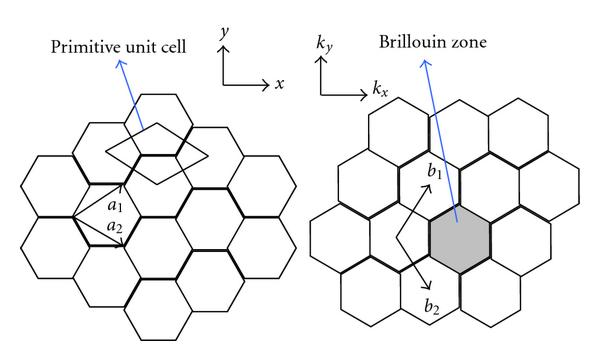
\includegraphics[scale=2]{BZ_Graphene.jpg}\end{center}
			\caption{Unit Cells for real and reciprocal space}
			\label{fig:unitcells}
			\end{figure}
			
			The distance between carbon atoms in real space is $a = 0.142$ nm, therefore we can see that the primitive lattice vectors are:
			
			\begin{center} $\textbf{a}_1 = \frac{a}{2} (3,\sqrt{3})$ and $\textbf{a}_2 = \frac{a}{2} (3,-\sqrt{3})$ \end{center}
			
			Taking the Fourier Transform of real space, we find that the lattice vectors for the reicprocal space are:
			
			\begin{center} $\textbf{b}_1 = \frac{2\pi}{3a} (1,\sqrt{3})$ and $\textbf{b}_2 = \frac{2\pi}{3a} (1,-\sqrt{3})$ \end{center}
			
			Starting with the assumption of a linear combination of atomic orbitals (LCAO), we find the ground state of an single electron $\psi_\textbf{k}(\textbf{r})$ moving through a potential of an isolated atom $U(\textbf{r})$.  We then notice that if the electrons are in the $s$ state and therefore have little affect on each other (i.e. the wavefunctions are linearly independent), then we can construct an approximate wavefunction for a single electron within the whole crystal lattice (rather than a single atom):
			\begin{equation}
				\Psi_\textbf{k}(\textbf{r}) = \sum_j C_{j\textbf{k}} \psi_\textbf{k}(\textbf{r})
			\end{equation}
			
			Where $j$ is each lattice point within the crystal.  We remember now that the solution to the Sch\"{o}dinger Equation for a periodic potential is of the Bloch function form (Kittel Equation 7.7):
			 
			\begin{equation}
				\psi_\textbf{k}(\textbf{r}) = u_\textbf{k}(\textbf{r}) e^{i\textbf{k}\cdot \textbf{r}}
			\end{equation}
			
			Now continuing with the scheme of Kittel Chapter 9, we see that $C_\textbf{k}(\textbf{r})=\frac{1}{\sqrt{N}}e^{i\textbf{k}\cdot\textbf{r}}$, and therefore:

			\begin{equation}
				\Psi_\textbf{k}(\textbf{r}) = \frac{1}{\sqrt{N}} \sum_j e^{i\textbf{k}\cdot\textbf{r}_j}\psi_\textbf{k}(\textbf{r}-\textbf{r}_j)
			\end{equation}

			Now to find the eigenenergies to te first order, we find the matrix elements for the crystal lattice:
			\begin{equation}
				\bra{\textbf{k}}H\ket{\textbf{k}} = \frac{1}{N} \sum_j \sum_m e^{i\textbf{k}\cdot(\textbf{r}_j-\textbf{r}_m)}\bra{\psi_m}H\ket{\psi_j}
			\end{equation}

			Where $\psi_m = \psi(\textbf{r}-\textbf{r}_m)$ and $\psi_j = \psi(\textbf{r}-\textbf{r}_j)$.  Now making the substitution $\boldsymbol{\rho}_m = \textbf{r}_m - \textbf{r}_j$:

			\begin{equation}
				\bra{\textbf{k}}H\ket{\textbf{k}} = \sum_m e^{-i\textbf{k}\cdot\boldsymbol{\rho}_j}\int \psi^*(\textbf{r}-\boldsymbol{\rho})H\psi(\textbf{r}) dV
			\end{equation}
			
			Now all integrals are neglected other than the ones on the same atom and the nearest neighbors (NN) which are connected by $\rho$ such that:
			
			\begin{equation}
				\int \psi^*(\textbf{r})H\psi(\textbf{r}) dV = -\alpha
			\end{equation}

			\begin{equation}
				\int \psi^*(\textbf{r}-\boldsymbol{\rho})H\psi(\textbf{r}) dV = -\gamma
			\end{equation}
			
			\begin{equation}
				\bra{\textbf{k}}H\ket{\textbf{k}} =\alpha  - \gamma \sum_m e^{-i\textbf{k}\cdot\boldsymbol{\rho}_m} = \boldsymbol{\epsilon}_k
			\end{equation}
			
			We see that the nearest neighbors for Graphene are:
			
			\begin{equation}
				\begin{aligned}
					\boldsymbol{\rho}_1 = \frac{a}{2}(1, \sqrt{3}) \\
					\boldsymbol{\rho}_2 = \frac{a}{2}(1, -\sqrt{3}) \\
					\boldsymbol{\rho}_3 = -a (1, 0) 
				\end{aligned}
			\end{equation}
			
			This gives the well known tight binding solution eigenenergies:
			
			\begin{equation}
				\bra{k}H\ket{k} = E_\pm (\textbf{k}) = \pm t \sqrt{3 + 2cos(\sqrt{3}k_ya) + 4cos(\frac{\sqrt{3}}{2}k_ya)cos(\frac{3}{2}k_xa)}
			\end{equation}
			
			This band structure can be shown in the first Brillouin zone with a simply python script:	\\
			\pagebreak
			\lstinputlisting[language=Python]{TightBindingGraphene.py}
			\pagebreak
			Which provides the following plots as it's output: \\
			
			\begin{figure}[!h]
				\subfloat[Fermi surface in first Brillouin Zone]{
				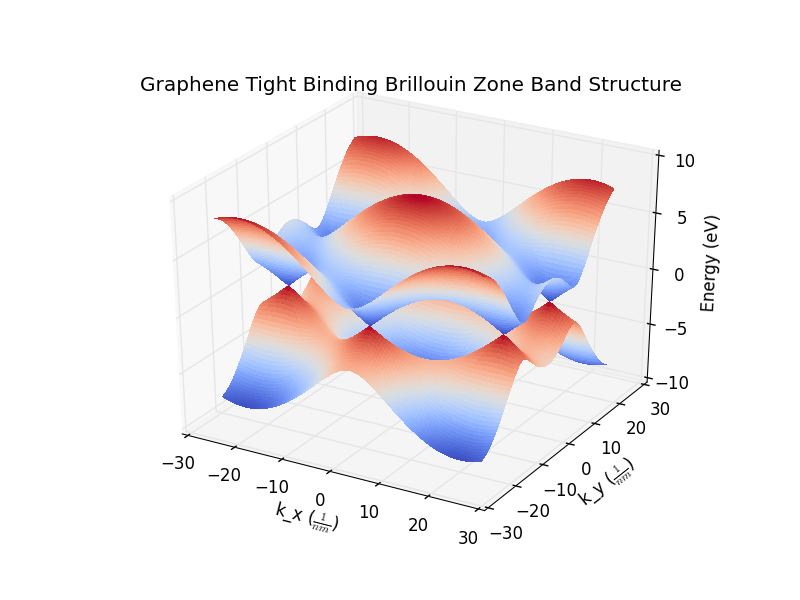
\includegraphics[scale=.4]{BZ_TightBinding.png}
				\label{fig:GrapheneTBBZ}
				}
				\subfloat[Dirac Cone Band strucutre around the K point]{
				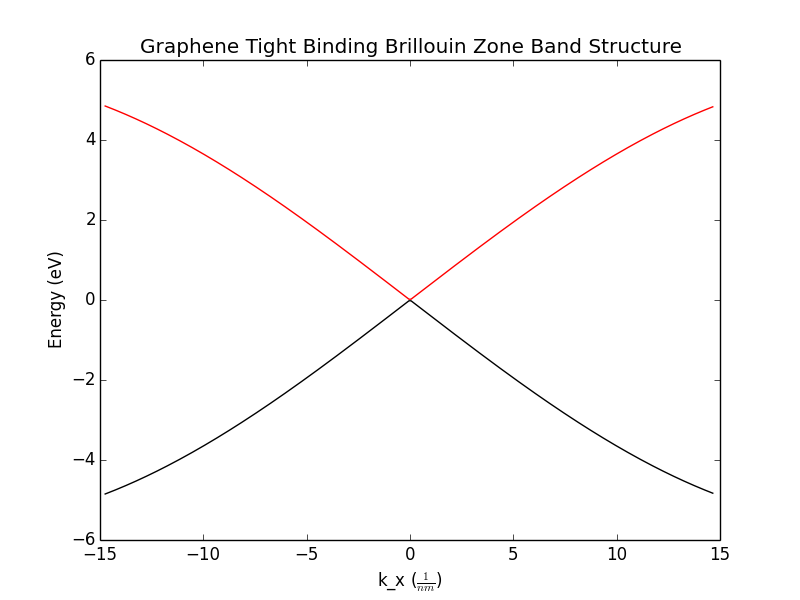
\includegraphics[scale=.4]{Kpoint_TightBinding.png}
				\label{fig:GrapheneTBKpoint}
				}
			\caption{Band structure of Graphene calculated with tight binding theory.}
			\label{fig:TBCalcs}
			\end{figure}
			
			
			\subsection{Comparison with ARPES data}
			
			We can see that the calculated band structure matches the band structure from the tight binding theory \textit{qualitatively}, by comparing Figure~\ref{fig:GrapheneTBKpoint} with Figure~\ref{fig:ARPES0}. 
			
			\begin{figure}[H]
				\centerline{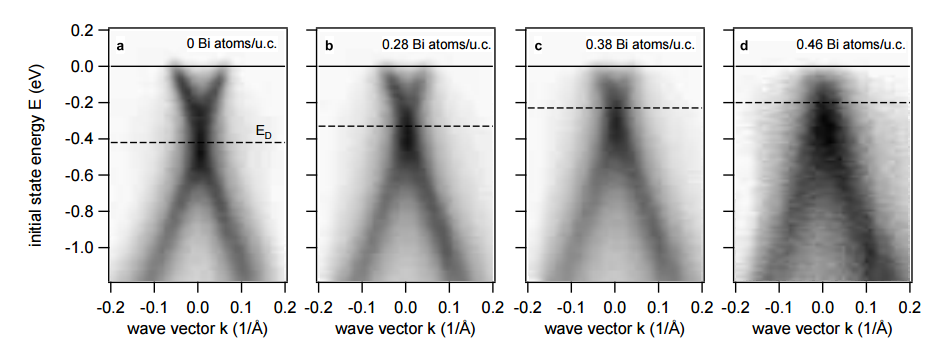
\includegraphics[scale=.7]{ARPESpaper.png}}
			\caption{ARPES of Graphene on SiC at various levels of doping.}
			\label{fig:ARPES0}
			\end{figure}
						
			\begin{figure}[H]
				\centerline{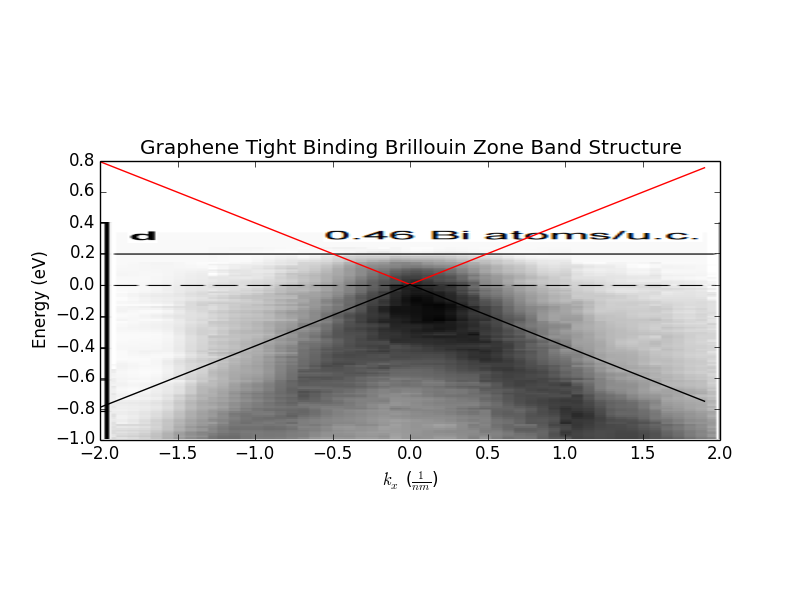
\includegraphics[width=9cm, height=15cm]{TBvsARPES46Bicent.png}}
			\caption{ARPES of Graphene with 0.46 Bismuth atoms per unit cell compared to tight binding theory.}
			\label{fig:TBARPESComp}
			\end{figure}
			
			However, the Fermi Level is shifted in the pristine graphene on SiC in Figure~\ref{fig:ARPES0}.  The study found that by doping the surface with Bismuth atoms, the Fermi level could approach the Dirac point, which would mimic free standing graphene which has it's intrinsic Fermi Level at the Dirac point at zero energy.  However, one note can be made about the curvature of the band structure which is more noticeable as the figures are overlayed, as in Figure~\ref{fig:TBARPESComp}.  This is due to the effective mass difference between what is considered in the tight binding theory and that of the effective mass in the real experiment.  Studies have been done which attempt to recover the curvature of this band through Fermi velocity renormalization in various scenarios for graphene and graphene related materials.\cite{elias2011dirac, attaccalite2009fermi, liu2012atlas}   \\
	~\
			
	~\	
	\pagebreak
	
			
			
	\bibliographystyle{acm}
	\bibliography{Homework10bib}
			
			
\end{homeworkProblem}

\end{document}
